\section{Atomic Structure Chain Operator protocol}
\label{app:atomStructUtilsOperatorProtocol}%a011
Protocol designed to perform two types of operations with chains from atomic structures in \scipion: a) Chain extraction: An individual chain will be extracted from a polymeric atomic structure. The extracted chain will be saved as monomer in a new atomic structure. b) Chain addition: One or several chains will be added to a reference atomic structure. The resulting addition will be saved as a new polymeric atomic structure. 

\begin{itemize}
 \item Requirements to run this protocol and visualize results:
    \begin{itemize}
        \item \scipion plugin: \ttt{scipion-em-atomstructutils}
        \item \scipion plugin: \ttt{scipion-em-chimera}
    \end{itemize}
 \item \scipion menu:
  \ttt{Protocols SPA -> Tools -> Calculators} (\ffigure{fig:app_protocol_atomstructutils_operator_1} (A))
  
 \item Protocol form parameters (\ffigure{fig:app_protocol_atomstructutils_operator_1} (B and C)):
 
 \begin{figure}[H]
     \centering 
     \captionsetup{width=.7\linewidth} 
     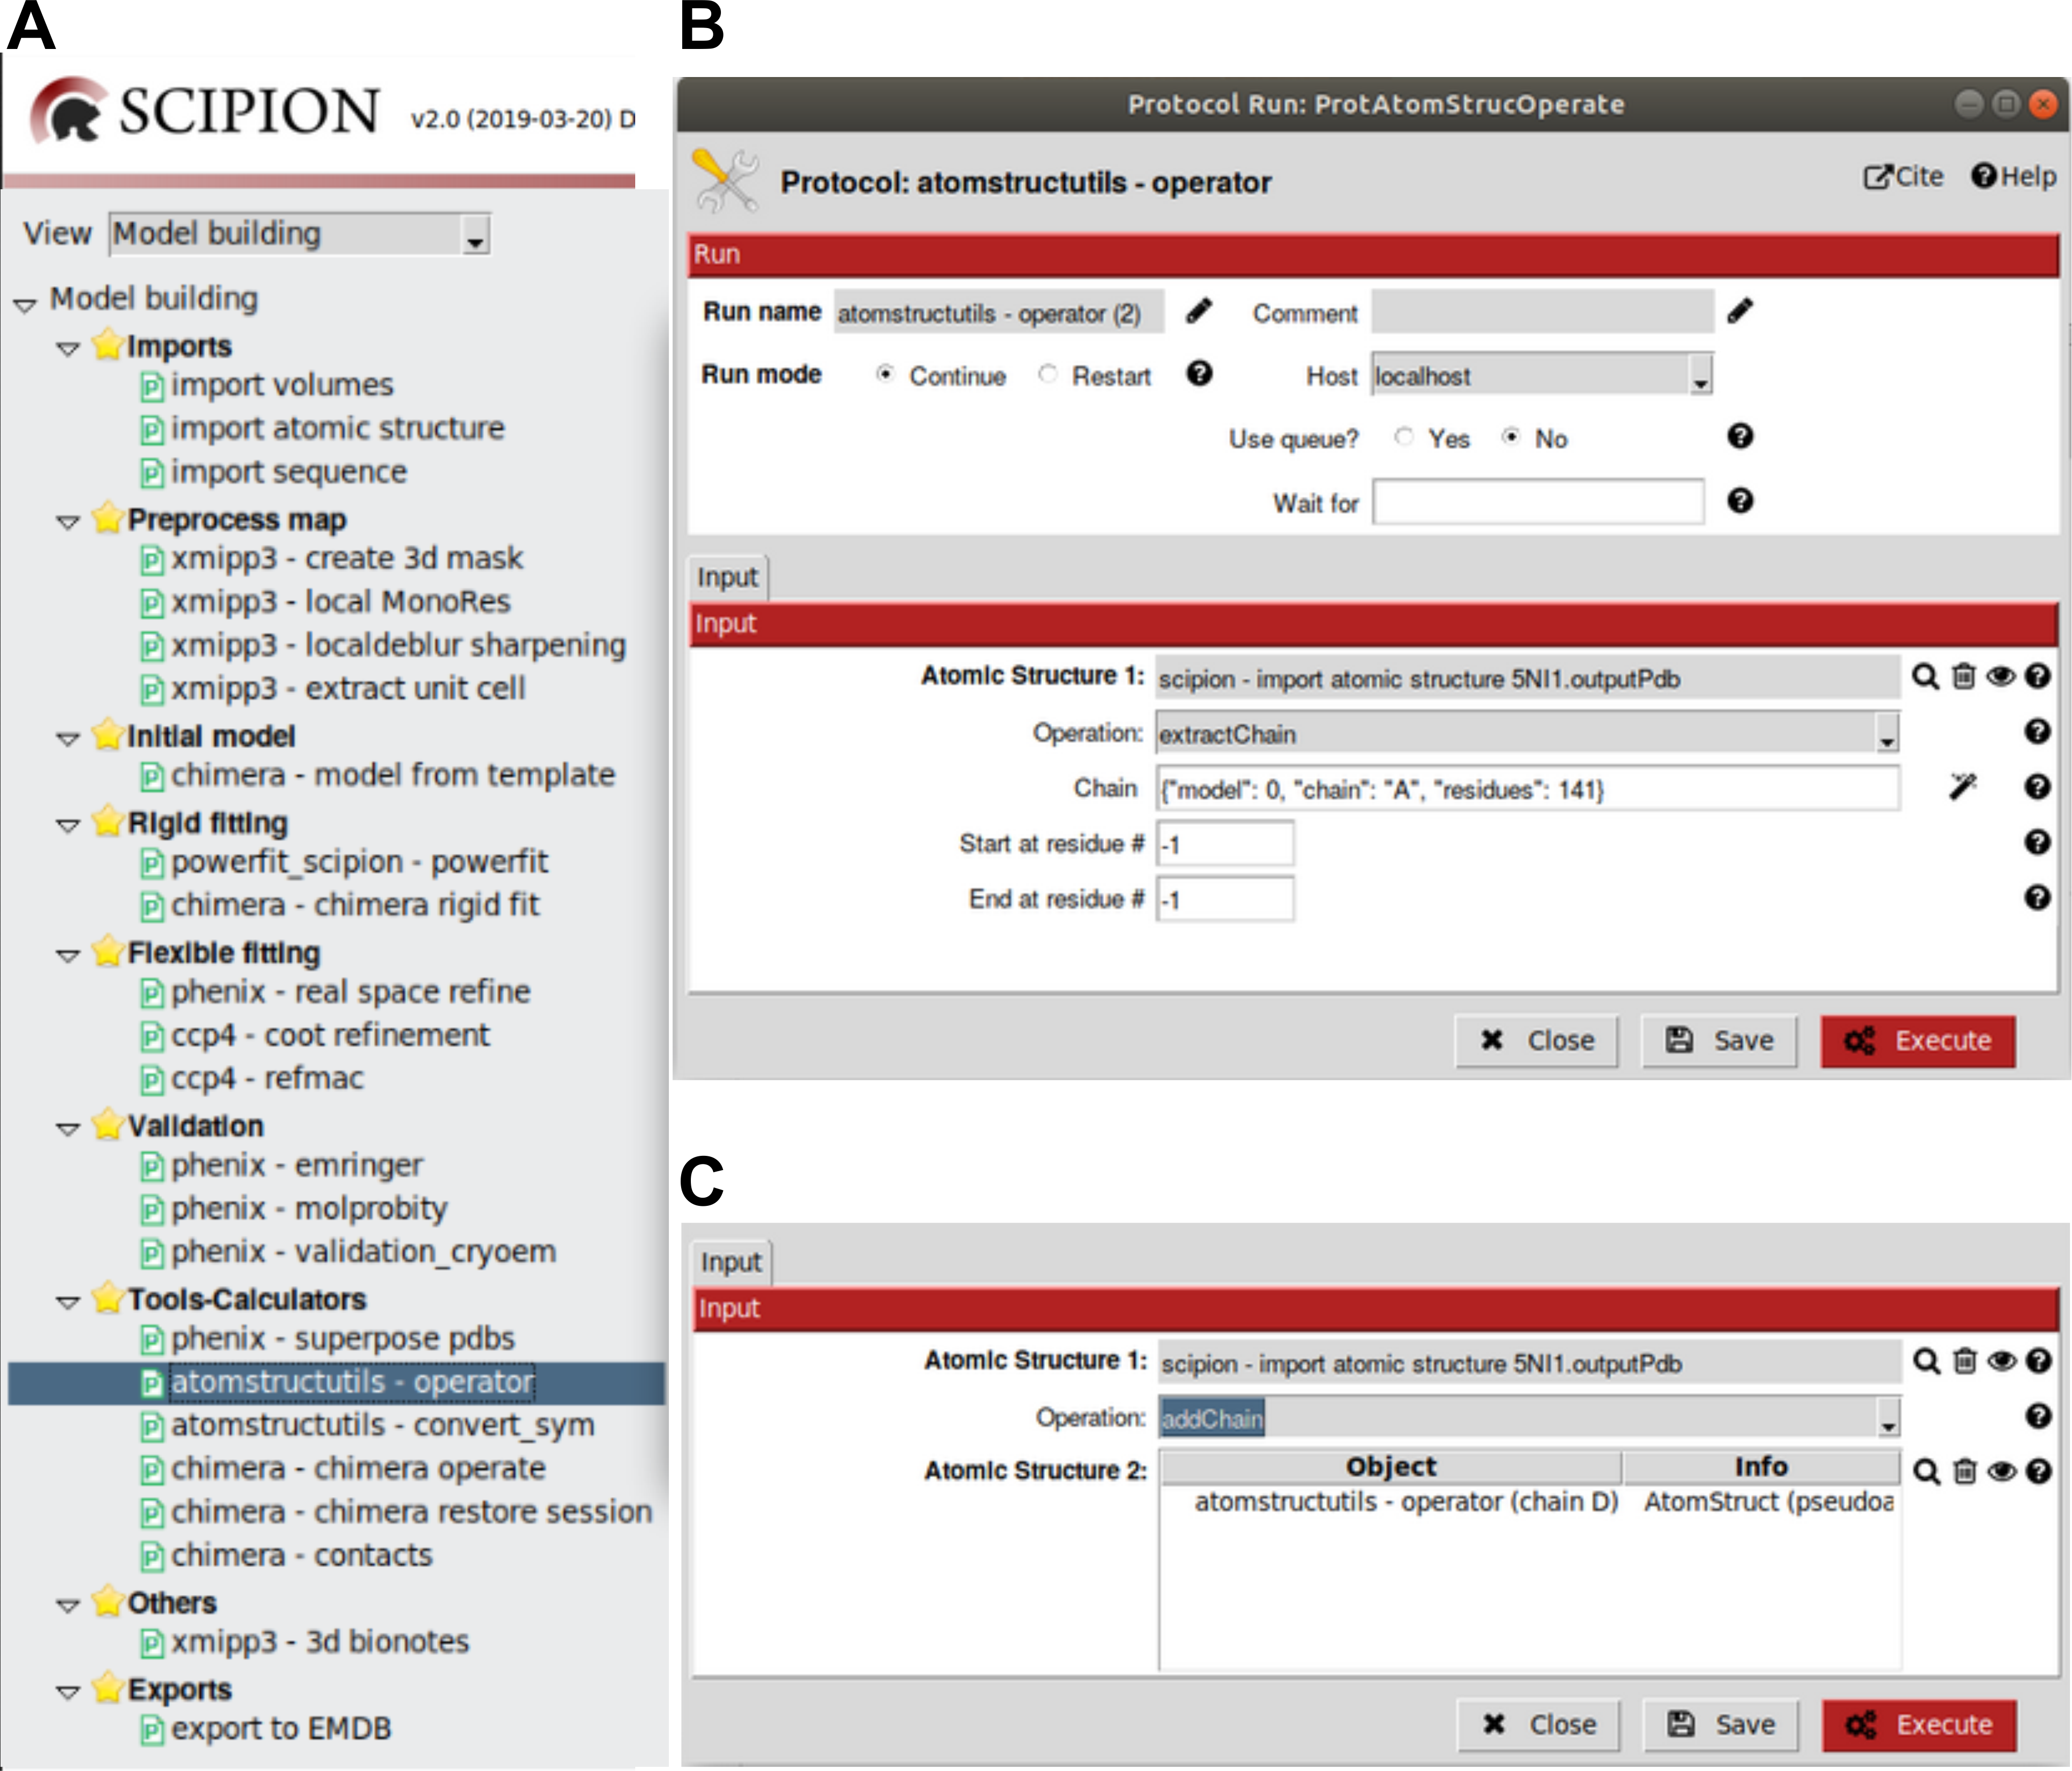
\includegraphics[width=0.90\textwidth]{Images_appendix/Fig154.pdf}
     \caption{Protocol \scommand{atomstructutils - operator}. A: Protocol location in \scipion menu. B: Protocol form to extract a chain from an atomic structure. C: Protocol form to add one or several chains to an atomic structure.}
     \label{fig:app_protocol_atomstructutils_operator_1}
    \end{figure}
    
   \begin{itemize}
    \item \ttt{Atomic structure 1}: PDBx/mmCIF atomic structure, previously downloaded or generated in \scipion. 
    \item \ttt{Operation}: Two types of operations can be performed with this protocol: 
    \begin{itemize}
     \item \ttt{extractChain}: Extraction of only one chain from a polymeric atomic structure. By selecting this option, three additional params have to be completed (\ffigure{fig:app_protocol_atomstructutils_operator_1} (B)):
     \begin{itemize}
      \item \ttt{Chain}: Specific chain that has to be extracted. The wizard on the right helps the user to select that chain showing the number of the starting model structure, the name of the chain, and its number of residues.
      \item \ttt{Start at residue \#}: The default value (-1) allows to extract the whole chain. In case you would like to extract only a fraction of the chain, the number of the initial required residue should be indicated. 
      \item \ttt{End at residue \#}: The default value (-1) allows to extract the whole chain. In case you would like to extract only a fraction of the chain, the number of the last required residue should be indicated. 
     \end{itemize}
     \item \ttt{addChain}: Addition of one or several chains to an initial atomic structure. By selecting this option, an additional param has to be completed (\ffigure{fig:app_protocol_atomstructutils_operator_1} (C)):
      \begin{itemize}
      \item \ttt{Atomic structure 2}: One or several PDBx/mmCIF atomic structures, previously downloaded or generated in \scipion.
      \end{itemize}
    \end{itemize}
   \end{itemize}
 
 \item Protocol execution:
 Adding specific structure/chain label is recommended in \ttt{Run name} section, at the form top. To add the label, open the protocol form, press the pencil symbol at the right side of \ttt{Run name} box, complete the label in the new opened window, press OK and, finally, close the protocol. This label will be shown in the output summary content (see below). If you want to run again this protocol, do not forget to set to \ttt{Restart} the \ttt{Run mode}.\\
  Press the \ttt{Execute} red button at the form bottom.
  
 \item Visualization of protocol results:
 
 After executing the protocol, press \ttt{Analyze Results} and \chimera graphics window will be opened by default. Atomic structures and volumes are referred to the origin of coordinates in \chimera. To show the relative position of atomic structure and electron density volume, the three coordinate axes are represented; X axis (red), Y axis (yellow), and Z axis (blue) (\ffigure{fig:app_protocol_volume_3}).  Coordinate axes and the new atomic structure generated are model numbers \ttt{\#0} and \ttt{\#1}, respectively, in \chimera \ttt{Model Panel}. Write in \chimera command line:\\
    \ttt{split \#1}\\
 to check the individual chains included in the new atomic structure generated.
    
 \item Summary content:\\
 Since an atomic structure is generated:

    \begin{itemize}
     \item Protocol output (below \scipion framework):\\
      \ttt{atomstructutils - operator -> ouputPdb}; \ttt{AtomStruct (pseudoatoms=True/ False, volume=True/ False)}.\\Pseudoatoms is set to \ttt{True} when the structure is made of pseudoatoms instead of atoms. Volume is set to \ttt{True} when an electron density map is associated to the atomic structure.
     \item \ttt{SUMMARY} box:\\No summary information.\\
    \end{itemize}
\end{itemize}

